{\fontsize{12pt}{22pt} \textbf{Neural network}\par}

\vspace{5mm}

While counting the layers, we usually don't include the input layer. The first schema (left) is a 1-layer neural network whereas the second schema (right) is a 2-layers neural network. We notice that a 1-layer neural network doesn't have any hidden layer.

\begin{center}
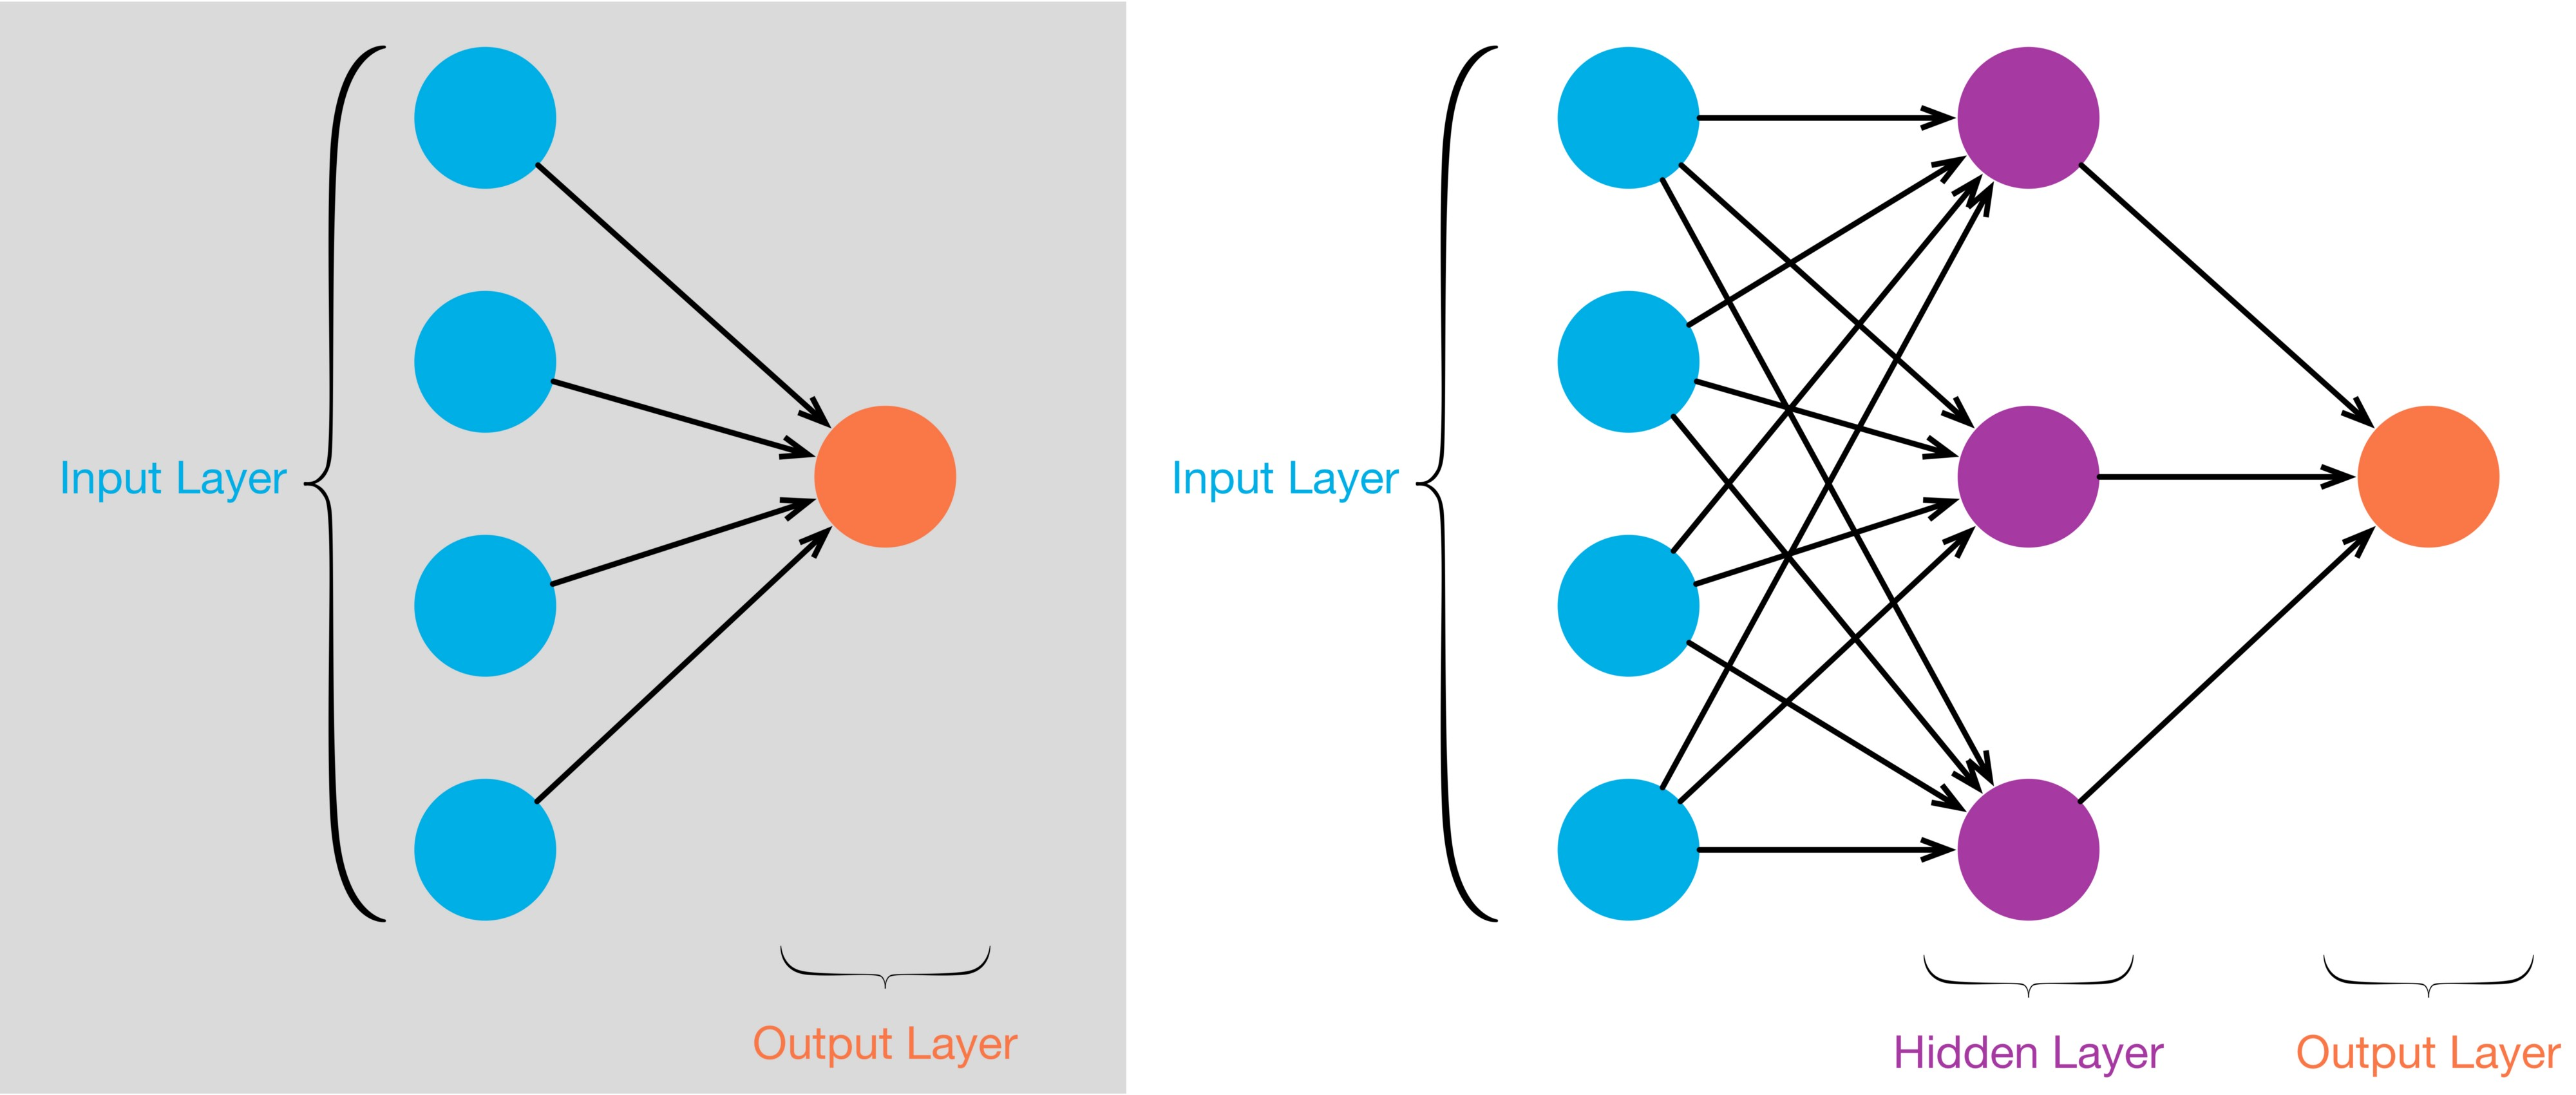
\includegraphics[scale=0.09]{nn-layers.jpeg}
\end{center}

\vspace{5mm}

\underline{1-layer neural network}

\vspace{5mm}

A 1-layer neural network can be seen as a logistic regression. The below explanation is largely inspired by  the example from coursera (\textit{deeplearning.ai})

Let us take the example of an image that we want to classify in a \textbf{binary} way: man/woman

The picture is vectorized as a vector of pixels : $\begin{pmatrix}x_1\\...\\x_p\end{pmatrix}$

We use a regression to predict if it's a man/woman:

$y=\omega^Tx + b$

Note: $x$ are all the pixels of \textbf{one} image.

\vspace{5mm}

We want a probability in output (if it's $\ge 0.5$ then we say it's a man).

We thus want the output to be $\widehat{y}=\sigma(\omega^Tx + b)=\mathbb{P}(y|x) \in [0,1]$

(see regression part to get more details on the sigmoid)

\vspace{5mm}

Now since it's a binary classification, we want the $y$ (real value) to be $0$ or $1$.

Thus, the loss function is:

$$\mathcal{L}(y, \widehat{y})=-[y\log(\widehat{y})+(1-y)\log(1-\widehat{y})]$$

We notice that the loss function increases when $y \neq \widehat y$.

\vspace{5mm}

The cost function is the empiric loss on all examples:

$$J(\omega, b)=\frac{1}{m}\Sigma_{i=1}^m\mathcal{L}(\widehat{y}^{(i)}, y^i)$$

\vspace{5mm}

\textit{Forward propagation}

$$x_1,x_2, \omega_1,\omega_2,b \to z=\omega_1x_1 + \omega_2x_2 + b \to \widehat{y}=a=\sigma(z) \to \mathcal{L}(a,y)$$

- First arrow: regression

- Second arrow: probability

- Third arrow: error

\vspace{5mm}

\textit{Backward propagation}

\vspace{5mm}

The idea is: with the error computed on the last step, we go backward in order to correct the parameters $\omega$ and $b$.

$$x_1,x_2, \omega_1,\omega_2,b \leftarrow z=\omega_1x_1 + \omega_2x_2 + b \leftarrow \widehat{y}=a=\sigma(z) \leftarrow \mathcal{L}(a,y)$$

To find the new value of $\omega$ we look for its change ($d \omega$) that we can obtain thanks to the \textbf{Chain rule}. It consists of decomposing the derivative into successive ones.

The parameters that are udpated during the training are the weights $\omega$ and the bias $b$. Thus we need to compute $\frac{d\mathcal{L}}{d\omega}="d\omega"$ and $\frac{d\mathcal{L}}{db}="db"$ . \\

First the weights:

$$d\omega=\frac{d\mathcal{L}}{da}\frac{da}{dz}\frac{dz}{d\omega}$$

$$\text{where:}$$

$$\frac{d\mathcal{L}}{da} = (\frac{d\mathcal{L}(a,y)}{da}) = -y \frac{1}{a} - (1-y) \frac{-1}{1-a} = \frac{1-y}{1-a} - \frac{y}{a} = \frac{(a-ay-y+ay)}{a(1-a)} = \frac{a-y}{a(1-a)}$$

$$\frac{da}{dz} = \frac{d \sigma(z)}{dz} = \frac{-(-1)e^{-z}}{(1+e^{-z})^2} = \frac{e^{-z}}{1+e^{-z}} \frac{1}{1+e^{-z}}= (1-\sigma(z))\sigma(z) = (1-a)a~~~~\text{Reminder: } \sigma(z) = \frac{1}{1+e^{-z}}$$

$$\frac{dz}{d\omega} = x$$

$$\text{Thus:}$$

$$\frac{d\mathcal{L}}{d\omega} = \frac{a-y}{a(1-a)}(1-a)ax = (a-y)x$$

Then the bias:

$$...$$

\textit{Note}: we can see that the updated weight depends on the previous prevision $a$. This is why it is necessary to recompute the predicted value at each iteration.

\lstset{language=Python}
\lstset{frame=lines}
\lstset{caption={Gradient descent (logistic regression with a NN mindset)}}
\lstset{label={lst:code_direct}}
\lstset{basicstyle=\footnotesize}
\begin{lstlisting}

for i in range(num_iterations):
        
     # Cost and gradient calculation
     grads, cost = propagate(w, b, X_train, Y_train) # propagation on ALL the training sample
        
     # Retrieve derivatives from grads
     dw = grads["dw"]
     db = grads["db"]
        
     # update parameters
     w = w - learning_rate * dw
     b = b - learning_rate * db
        
     # Record the costs
     costs.append(cost)

\end{lstlisting}

\lstset{language=Python}
\lstset{frame=lines}
\lstset{caption={Propagation (logistic regression with a NN mindset)}}
\lstset{label={lst:code_direct}}
\lstset{basicstyle=\footnotesize}
\begin{lstlisting}
def propagate(w, b, X, Y):
    
    m = X.shape[1]
    
    # FORWARD PROPAGATION (FROM X TO COST)
    A = sigmoid(np.dot(w.T,X)+b)
    cost = (- 1 / m) * np.sum(Y * np.log(A) + (1 - Y) * (np.log(1 - A))
    
    # BACKWARD PROPAGATION (TO FIND GRAD)
    dw = (1/m)*np.dot(X,(A-Y).T)
    db = (1/m)*np.sum(A-Y)

\end{lstlisting}



\vspace{5mm}